\begin{flushright} {\tiny {\color{gray} solvers.tex}} \end{flushright}
%~~~~~~~~~~~~~~~~~~~~~~~~~~~~~~~~~~~~~~~~~~~~~~~~~~~~~~~~~~~~~~~~~~~~~~~~~~~~~~~~~~~~~~~~~~~~~~~~~~

Let us start again from the (full) Stokes system:
\begin{equation}
\underbrace{
\left(
\begin{array}{cc}
\K & \G \\ \G^T & -\C 
\end{array}
\right)
}_{\cal A}
\cdot
\left(
\begin{array}{c}
\vec{\cal V} \\ \vec{\cal P}
\end{array}
\right)
=
\left(
\begin{array}{c}
\vec{f} \\ \vec{h}
\end{array}
\right)
\label{StokesSyst}
\end{equation}
We need to solve this system in order to obtain the solution, i.e. the $\vec{\cal V}$ 
and $\vec{\cal P}$ vectors. But how? 
Unfortunately, this question is not simple to answer and the appropriate method depends on many 
parameters, but mainly on how big the matrix blocks are and what the condition number of the matrix $\K$ is. 

First let us start with an obvious question: couldn't we just compute the inverse of the matrix ${\cal A}$?
Under the assumption that the inverse of $\K$ and $\SSS$ exists, we can and we find\footnote{The matrix 
$\C$ is here omitted but it bears no consequences on the conclusion.}
\[
{\cal A}^{-1} = 
\left(
\begin{array}{cc}
\K & \G \\ \G^T & 0
\end{array}
\right)^{-1}
=
\left(
\begin{array}{cc}
\K^{-1} + \K^{-1} \cdot \G \cdot\SSS^{-1} \cdot\G^T \cdot\K^{-1} & -\K^{-1} \cdot\G \cdot\SSS^{-1} \\ 
-\SSS^{-1} \cdot\G^T \cdot\K^{-1}  &  \SSS^{-1}
\end{array}
\right)
\]
However, such an expression is of limited interest in the numerical solution of saddle
point problems since it showcases 5 times the inverse of $\K$ and more importantly
the inverse of the Schur complement matrix $\S$ which is likely to be a full matrix so 
that we never want to compute it explicitely.


As concisely explained in Clevenger \& Heister (2021) \cite{clhe21}, 
there are three common approaches used in the literature for solving the above equation on large scales:
\begin{itemize}
\item a pressure corrected, Schur complement CG scheme, using multigrid as an 
approximation to the velocity block;
\item a block-preconditioned Krylov
method, also using multigrid on the velocity block.
For this method, there are two main types:
\begin{itemize}
\item GMRES\cite{mabl15,rumi15} (or any Krylov method not requiring symmetry) with
block-triangular preconditioner (This is what \aspect does):
\[
{\bm P} = \left(
\begin{array}{cc}
\K & \G \\
0 & - \SSS
\end{array}
\right)
\]

\item MINRES\cite{gmhj16} with block-diagonal preconditioner
\[
{\bm P} = \left(
\begin{array}{cc}
\K & 0 \\
0 & - \SSS
\end{array}
\right)
\]

\end{itemize}


\item an all-at-once multigrid performed on the entire Stokes
system, using Uzawa-type smoothers.
\end{itemize}


\Literature: Preconditioners for Incompressible Navier-Stokes Solvers \cite{seuv10}

Saddle point preconditioners have been extensively discussed and studied \cite{bewa08}, \cite{dewu04}

Diagonal preconditioners in \cite{shrb01}, \cite{babc94}.



%...................................................
\subsubsection{When using the penalty formulation}

In this case we are only solving for 
velocity since pressure has been eliminated and is later recovered in a post-processing step:
\[
(\K_\eta+\K_\lambda) \cdot \vec {\cal V} = \vec f
\]
 We also know that 
the penalty factor $\lambda$ is many orders of magnitude higher than the viscosity and 
in combination with the use of the $Q_1 \times P_0$ element the resulting matrix 
condition number is very high so that the use of iterative solvers is precluded. 
Indeed codes such as \sopale \cite{full95}, \douar \cite{brtf08}, \fantom \cite{thie11} 
or \sulec \cite{qube11} relying on the penalty formulation all use direct solvers.
The most popular are BLKFCT\footnote{\url{http://dm.unife.it/blkfclt/}}, 
MUMPS\footnote{\url{http://mumps.enseeiht.fr/}}\cite{amdu89,amdl00,amdk01,amgl06,ambl19}, 
PasTiX \cite{herr02},
WSMP\footnote{\url{http://www.research.ibm.com/projects/wsmp}} \cite{GUPTA94ieee,GUPTA09sc-long},
UMFPACK and CHOLMOD\footnote{\url{http://faculty.cse.tamu.edu/davis/suitesparse.html}}
, SuperLU\footnote{\url{https://portal.nersc.gov/project/sparse/superlu/}}, 
PARDISO\footnote{\url{https://www.pardiso-project.org/}}
\cite{pardiso-6.0a,pardiso-6.0b,pardiso-6.0c}, or those inside 
PETSc\footnote{\url{https://www.mcs.anl.gov/petsc/}}.

Braun \etal (2008) \cite{brtf08} list the following features of direct solvers:
\begin{itemize}
\item Robust
\item Black-box operation
\item Difficult to parallelize
\item Memory consumption
\item Limited scalability
\end{itemize}

The main advantage of direct solvers is used in this case: They can solve ill-conditioned 
matrices. However, memory requirements for the storage of number of nonzeros in the 
Cholesky matrix grow very fast as the number of equations/grid size increases, especially in 3D,
to the point that even modern computers with tens of Gb of RAM cannot deal with a $\sim 100^3$ element mesh.
This explains why direct solvers are often used for 2D problems and rarely in 3D with noticeable 
exceptions \cite{thfb08,yahb09,brya10,lobh10,alht11,alht12,alhf13,whbb14,neew18}. 

%....................................................................
\subsubsection{Uzawa algorithms and the Schur complement approach }

\index{general}{Uzawa algorithm}

Let us write the above system as two equations:
\begin{eqnarray}
\K \cdot \vec{\cal V} + \G \cdot \vec{\cal P} &=& \vec{f} \\
\G^T \cdot  \vec{\cal V} - \C \cdot \vec{\cal P} &=& \vec{h} 
\end{eqnarray}
The first line can be re-written 
$\vec{\cal V}=\K^{-1}\cdot (\vec{f} - \G \cdot \vec{\cal P})$ and can be inserted in the second:
\begin{equation}
\G^T\cdot \vec{\cal V} =\G^T \cdot  [ \K^{-1} \cdot  (\vec{f} - \G \cdot  \vec{\cal P}) ] - \C\cdot \vec{\cal P} = \vec{h} 
\end{equation}
or, 
\begin{mdframed}[backgroundcolor=blue!5]
\begin{equation}
(\G^T \cdot \K^{-1} \cdot \G + \C) \cdot \vec{\cal P} = \G^T \cdot \K^{-1}\cdot \vec{f} - \vec{h} 
\end{equation}
\end{mdframed}
The matrix $\SSS= \G^T \cdot \K^{-1} \cdot \G + \C$ is called the Schur complement. 
\index{general}{Schur Complement} 
It is Symmetric (since $\K$ is symmetric) and  Positive-Definite\footnote{$M$ 
positive definite $\iff$ $x^TMx>0$ $\forall \; x\in \mathbb{R}^n \setminus {\bm 0}$ }
(SPD) \index{general}{SPD} if $Ker({\G})=0$. 
Having solved this equation (i.e. we have obtained $\vec{\cal P}$), the velocity can be recovered by solving 
$\K\cdot \vec{\cal V} =\vec{f}- \G \cdot \vec{\cal P}$. 

\begin{remark}
The Schur complement matrix naturally occurs when the Stokes matrix is decomposed using 
a LDU block-factorisation. Indeed, we have 
\[
\left(
\begin{array}{cc}
\K & \G \\ 
\G^T & 0
\end{array}
\right)
=
\left(
\begin{array}{cc}
{\bm I} & 0 \\ 
\G^T \cdot \K^{-1} & {\bm I}
\end{array}
\right)
\cdot
\left(
\begin{array}{cc}
\K & 0 \\ 
0 & -\SSS
\end{array}
\right)
\cdot
\left(
\begin{array}{cc}
{\bm I} & \K^{-1} \cdot \G \\ 
0 & {\bm I}
\end{array}
\right)
\]
\end{remark}

For now, let us assume that we have built the $\SSS$ matrix\footnote{We will 
revisit this topic later on, but be aware that we never build $\SSS$ in practice.} 
and the right hand 
side $\underline{\vec{f}}=\G^T \cdot \K^{-1} \cdot \vec{f} - \vec{h}$.
We must solve $\SSS\cdot \vec{\cal P} = \underline{\vec{f}}$.
It is easy to see that $\SSS$ is actually a full matrix (i.e. not sparse) and 
aside from the costs of building it explicitly using a direct solver would require 
a lot of memory so that we must then turn to iterative methods. 

\index{general}{Richardson Iterations}
One can resort to so-called Richardson iterations, defined as follows 
(e.g., see Varga \cite{varga}, p141):
in solving the matrix equation ${\bm A}\cdot {\vec X}={\vec b}$,
the Richardson iterative method is defined by: 
\begin{equation}
{\vec X}_{k+1} = {\vec X}_k + \alpha_k (-{\bm A} \cdot {\vec X}_k + {\vec b})
\quad\quad
m\geq 0 
\end{equation}
where the $\alpha_k$'s are real scalars. 
It is easy to see that when the method converges then ${\vec X}_{k+1} \simeq {\vec X}_k$  and then 
for $\alpha_k\neq 0$ then ${\bm A}\cdot {\vec X}={\vec b}$ is satisfied. 
In our case, it writes:
\begin{eqnarray}
\vec {\cal P}_{k+1} 
&=& \vec {\cal P}_{k} + \alpha_k ( - \SSS \cdot \vec{\cal P}_{k}  +  \underline{\vec{f}}) \nonumber\\
&=& \vec {\cal P}_{k} + \alpha_k \left[ - (\G^T \cdot \K^{-1} \cdot \G + \C)  \cdot \vec{\cal P}_{k} 
+  (\G^T \cdot \K^{-1} \cdot \vec{f} - \vec{h}   ) \right] \nonumber\\
&=& \vec {\cal P}_{k} + \alpha_k \left[ \G^T \cdot \K^{-1} \cdot ( - \G \cdot \vec{\cal P}_{k} + \vec{f}) 
-\C \cdot \vec{\cal P}_{k} - \vec{h} 
\right] \nonumber\\
&=& \vec {\cal P}_{k} + \alpha_k \left[ \G^T \cdot \K^{-1} \cdot ( \K\cdot \vec{\cal V}_k)
-\C \cdot \vec{\cal P}_{k}  - \vec{h} \right] \nonumber\\
&=& \vec {\cal P}_{k} + \alpha_k \left( \G^T \cdot \vec{\cal V}_k -\C \cdot \vec{\cal P}_{k} - \vec{h} \right) 
\end{eqnarray}
The above iterations are then carried out and for each new pressure field the associated velocity field 
is computed. The method of using Richardson iterations applied to the Schur complement 
is commonly called the Uzawa algorithm (see Braess \cite[p221]{braess}
\footnote{I have slightly 
altered the indices of the velocities wrt the book}).

\begin{mdframed}[backgroundcolor=blue!5]
\underline{\bf Uzawa algorithm (1)}: assume $\vec{\cal P}_0$ known
\begin{eqnarray}
\text{solve} \qquad \mathbb{K} \cdot \vec{\cal V}_k &=& \vec f - \mathbb{G}\cdot \vec {\cal P}_{k} \\
\vec{\cal P}_{k+1} &=& 
\vec{\cal P}_{k}  + \alpha_k (\mathbb{G}^T\cdot \vec{\cal V}_k  -\C \cdot \vec{\cal P}_{k} -\vec h)
\quad
\quad
\quad
\quad
k=0,1,2, ... \label{uzaa2}
\end{eqnarray}
\end{mdframed}


This method is rather simple to implement, although
what makes an appropriate set of $\alpha_k$ values is not straightforward, which is why 
the conjugate gradient is often preferred, as detailed in the next section. 

It is known that such iterations will converge for $0< \alpha < \rho(\SSS)= \lambda_{max}(\SSS)$ 
where $\rho(\SSS)$ is the spectral radius of the matrix $\SSS$
which is essentially the largest, in absolute value, eigenvalue of $\SSS$ (neither of which 
can be computed easily).  
It can also be proven that the rate of convergence depends on the condition number of the matrix.

Richardson iterations are part of the family of stationary iterative 
methods\footnote{\url{https://mathworld.wolfram.com/StationaryIterativeMethod.html}}, 
since it can be rewritten 
\begin{equation}
{\vec X}_{k+1} = ({\bm I} - \alpha_k {\bm A} ) \cdot {\vec X}_k + \alpha_k {\vec b}
\end{equation}
which is the definition of a stationary method. 
The four main stationary methods are the Jacobi method, 
Gauss-Seidel method, successive overrelaxation method (SOR), 
and symmetric successive overrelaxation method (SSOR)
\index{general}{Jacobi Iterative Method}
\index{general}{Gauss-Seidel Iterative Method}
\index{general}{SOR Iterative Method}
\index{general}{SSOR Iterative Method}


Since the $\alpha$ parameter is the key to a successful Uzawa algorithm, 
this issue has of course been looked into. What follows is 
presented in p221 of Braess \cite{braess}.
For the analysis of the Uzawa algorithm, we define the residue
\[
\vec {\cal R}_k = \vec h - \mathbb{G}^T \cdot \vec{\cal V}_k  +\C \cdot \vec{\cal P}_{k}
\]
In addition, suppose the solution of the saddle point problem is denoted
by $(\vec{\cal V}^\star,\vec{\cal P}^\star)$ so that we have
\[
\vec{f} = \K \cdot \vec{\cal V}^\star + \G \cdot \vec{\cal P}^\star
\qquad
{\rm and}
\qquad
\vec{h} = \G^T \cdot \vec{\cal V}^\star - \C \cdot \vec{\cal P}^\star 
\]

Now substituting the iteration formula for ${\cal V}_k$, and inserting $\vec{f}$ and $\vec{h}$ from above,
we get
\begin{eqnarray}
\vec{\cal R}_k 
&=& \vec{h} -\G^T  \cdot \vec{\cal V}_k  +\C \cdot \vec{\cal P}_{k} \nn\\
&=& \vec{h} -\mathbb{G}^T\cdot \mathbb{K}^{-1} (\vec f - \mathbb{G}\cdot \vec{\cal P}_{k})  +\C \cdot \vec{\cal P}_{k}\\
&=& (\G^T\cdot\vec{\cal V}^\star - \C \cdot \vec{\cal P}^\star) -\mathbb{G}^T\cdot \mathbb{K}^{-1} (\K\cdot\vec{\cal V}^\star 
+ \G\cdot\vec{\cal P}^\star - {\G}\cdot \vec{\cal P}_{k})+\C \cdot \vec{\cal P}_{k} \\
&=& ({\G}^T \cdot \mathbb{K}^{-1} \cdot \mathbb{G} + \C)\cdot (\vec {\cal P}_{k} - \vec{\cal P}^\star) 
\end{eqnarray}
From Eq.~\eqref{uzaa2} it follows that:
\begin{eqnarray}
\vec{\cal P}_{k+1} - \vec{\cal P}_{k}  
&=& \alpha\; (\mathbb{G}^T\cdot \vec{\cal V}_k -\C \cdot \vec{\cal P}_{k} -\vec h) \\
&=& -\alpha\; \vec{\cal R}_k \\ 
&=& -\alpha\; ( \mathbb{G}^T \cdot \mathbb{K}^{-1} \cdot \mathbb{G} + \C )
\cdot (\vec {\cal P}_{k} -\vec{\cal P}^\star)\\ 
&=& \alpha\; (\mathbb{G}^T \cdot \mathbb{K}^{-1} \cdot \mathbb{G} + \C) \cdot 
(\vec{\cal P}^\star - \vec {\cal P}_{k} ) 
\end{eqnarray}
Thus the Uzawa algorithm is equivalent to applying the gradient method 
to the reduced equation using a fixed step size. 
In particular, the iteration converges for
$
\alpha < 2 || \G^T \cdot \K^{-1} \cdot \G + \C||^{-1}
$
and one can show that the good step size $\alpha_k$ is given by 
\begin{equation}
\alpha_k = \frac{\vec{\cal R}_k \cdot \vec{\cal R}_k}
{(\G \cdot \vec{\cal R}_k)\cdot (\K^{-1}\cdot \G \cdot \vec{\cal R}_k)}
\label{uzaa3}
\end{equation}
\todo[inline]{include matrix $\C$!}


However, if we were to use this rule formally, we would 
need an additional multiplication by $\K^{-1}$ in every step 
of the iteration. This can be avoided by storing an 
auxiliary vector. 
Note that this algorithm is presented in Zienkiewicz \etal (1985) \cite{zivt85} 
in the context of viscoplastic flow.

%Note that in \cite{glow} it is stated: the convergence of this algorithm is proved for 
%$\alpha \in (0,2\mu/d)$ (where $d$ is the number of dimensions).
%\todo[inline]{check this, and report page number}

As mentioned above, there is a way to rework the original Uzawa algorithm 
to include Eq. (\ref{uzaa3}). It is yields a modified 
Uzawa algorithm (see p222 of Braess \cite{braess}
\footnote{I have slightly 
altered the indices of the velocities wrt the book}):


\begin{mdframed}[backgroundcolor=blue!5]
\underline{\bf Uzawa algorithm (2)}: assume $\vec{\cal P}_0$ known. 
Solve $\mathbb{K}\cdot \vec{\cal V}_0 = \vec f - \mathbb{G}\cdot  \vec{\cal P}_0$. 
For $k=0,1,2,...$, compute 
\begin{eqnarray}
\vec{\cal R}_k=\vec q_k &=& \vec h-\mathbb{G}^T \cdot \vec{\cal V}_k + \C \cdot \vec{\cal P}_{k}\\
\vec{p}_k &=& {\G}\cdot q_k \\
\vec H_k &=& {\K}^{-1}\cdot \vec{p}_k \\
\alpha_k &=& \frac{\vec q_k \cdot \vec q_k}{\vec{p}_k \cdot \vec H_k} \\
\vec {\cal P}_k &=& \vec {\cal P}_{k-1} - \alpha_k  \vec q_k \\
\vec {\cal V}_{k} &=& \vec {\cal V}_{k-1} + \alpha_k  \vec H_k
\end{eqnarray}
\end{mdframed}


\Literature: Cahouet \& Chabard (1988) \cite{cach88}, Cao (2003) \cite{cao03}.





%...................................................
\subsubsection{Conjugate gradient and the Schur complement approach }
\label{ss:schurpcg}

\index{general}{CG} \index{general}{Conjugate Gradient}
Since the Schur matrix $\SSS$ is Symmetric Positive Definite, 
the Conjugate Gradient (CG) method\footnote{\url{https://en.wikipedia.org/wiki/Conjugate_gradient_method}} \cite{hest52} 
is very appropriate to solve this system. 

Indeed, looking at the definition of Wikipedia: "{\it In mathematics, the conjugate gradient method is an algorithm 
for the numerical solution of particular systems of linear equations, namely those whose matrix is symmetric and positive-definite. 
The conjugate gradient method is often implemented as an iterative algorithm, applicable to sparse systems that are too large 
to be handled by a direct implementation or other direct methods such as the Cholesky decomposition. 
Large sparse systems often arise when numerically solving partial differential equations or optimization problems.}"

A simple Google search tells us that the Conjugate Gradient algorithm is as follows:

\begin{minipage}{0.40\textwidth}
\centering
{\captionfont Algorithm as obtained from Wikipedia.}\\
\frame{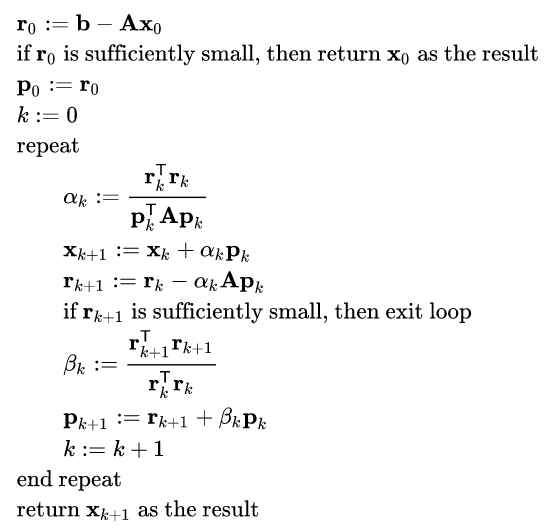
\includegraphics[width=7cm]{images/solvers/cgwiki}}
\end{minipage}\hfill
\begin{minipage}{0.50\textwidth}
The same algorithm with our notations:\\
$\vec{r}_0 = \underline{\vec{f}} - \SSS \cdot \vec{\cal P}_0$\\
$\vec{p}_0 = \vec{r}_0$\\
$k=0$ \\
repeat\\
\hspace{8mm} $\alpha_k = (\vec{r}_k^T\cdot \vec{r}_k )/(\vec{p}_k \cdot \SSS\cdot  \vec{p}_k )$\\
\hspace{8mm} $\vec{\cal P}_{k+1} = \vec{\cal P}_k+\alpha_k \vec{p}_k$\\
\hspace{8mm} $\vec{r}_{k+1} = \vec{r}_k - \alpha_k \; \SSS \cdot \vec{p}_k $ \\
\hspace{8mm} $\beta_k=(\vec{r}_{k+1}^T \cdot \vec{r}_{k+1})/(\vec{r}_k^T \cdot \vec{r}_k)$ \\
\hspace{8mm} $\vec{p}_{k+1} =\vec{r}_{k+1}+ \beta_k \vec{p}_k$ \\
$k=k+1$ \\
end repeat\\
return $\vec{\cal P}_{k+1}$ as the result
\end{minipage}

\vspace{.5cm}

This algorithm is of course explained in detail in many textbooks such as Saad \cite{saad},
in Zhong, Yuen, Moresi \& Knepley (2012) \cite{zhym12}, and in Section~\ref{ss:itsolvers}.

Let us look at this algorithm more closely. The parts which may prove to be somewhat tricky 
are those involving the matrix the Schur complement matrix since we wish never to build 
it explicitely. We start the iterations with a guess pressure $\vec{\cal P}_0$ (and an initial guess velocity 
which could be obtained by 
solving $\K\cdot \vec{\cal V}_0 =\vec{f}- \G\cdot \vec{\cal P}_0$).
\begin{eqnarray}
\vec{r}_0 
&=& \underline{\vec{f}}-\SSS \cdot \vec{\cal P}_0 \\
&=& \G^T\cdot \K^{-1}\cdot \vec{f} - \vec{h} - (\G^T\cdot \K^{-1}\cdot \G + \C)\cdot \vec{\cal P}_0 \\ 
&=& \G^T\cdot \K^{-1}\cdot (\vec{f} - \G\cdot \vec{\cal P}_0) - \vec{h} \\
&=& \G^T\cdot \K^{-1}\cdot \K\cdot \vec{\cal V}_0 -\C \cdot \vec{\cal P}_0 - \vec{h} \\ 
&=& \G^T\cdot \vec{\cal V}_0  -\C \cdot \vec{\cal P}_0   - \vec{h} 
\end{eqnarray}
We see that we were able to compute $\SSS \cdot \vec{\cal P}_0$ without ever forming the 
Schur complement matrix explicitely. We now turn to the $\alpha_k$ coefficient:
\[
\alpha_k 
= \frac{\vec{r}_k^T\cdot \vec{r}_k }{\vec{p}_k \cdot \SSS\cdot  \vec{p}_k } 
= \frac{\vec{r}_k^T \cdot \vec{r}_k }{\vec{p}_k\cdot (\G^T \cdot \K^{-1} \cdot \G +\C )\cdot \vec{p}_k } 
= \frac{\vec{r}_k^T \cdot \vec{r}_k }{(\G\cdot \vec{p}_k)^T \cdot  \K^{-1} \cdot (\G \cdot \vec{p}_k) + \vec{p}_k\cdot \C\cdot \vec{p}_k } 
\]
We then define $\tilde{\vec{p}}_k = \G \cdot \vec{p}_k$, so that $\alpha_k$ can be computed as follows:
\begin{enumerate}
\item compute $\tilde{\vec{p}}_k = \G \cdot  \vec{p}_k$
\item solve $\K\cdot  \vec{d}_k = \tilde{\vec{p}}_k$
\item compute 
\[
\alpha_k=\frac{\vec{r}_k^T \cdot \vec{r}_k}{\tilde{\vec{p}}_k^T \cdot \vec{d}_k 
+ \vec{p}_k\cdot \C\cdot \vec{p}_k }
\]
\end{enumerate}
Then we need to look at the term $\SSS\cdot \vec{p}_k$:
\[
\SSS\cdot \vec{p}_k = (\G^T\cdot \K^{-1}\cdot \G\cdot +\C )\vec{p}_k 
= \G^T\cdot \K^{-1}\cdot \tilde{\vec{p}}_k  + \C\cdot \vec{p}_k= \G^T\cdot  \vec{d}_k + \C \cdot \vec{p}_k
\]
We can then rewrite the CG algorithm as follows: 
\begin{itemize}
\item choose $\vec{\cal P}_0$
\item compute $\vec{\cal V}_0$ solution of $\K\cdot \vec{\cal V}_0 =\vec{f}- \G\cdot \vec{\cal P}_0$ 
\item $\vec{r}_0 = \G^T\cdot \vec{\cal V}_0 - \C \cdot \vec{\cal P}_0 - \vec{h}$ 
\item if $\vec{r}_0$ is sufficiently small, then return $(\vec{\cal V}_0,\vec{\cal P}_0)$ as the result
\item $\vec{p}_0=\vec{r}_0$
\item $k=0$
\item repeat
\begin{itemize}
\item compute $\tilde{\vec{p}}_k = \G\cdot \vec{p}_k$
\item solve $\K\cdot  \vec{d}_k = \tilde{\vec{p}}_k$
\item compute $\alpha_k=(\vec{r}_k^T \cdot  \vec{r}_k)/
              (\tilde{\vec{p}}_k^T\cdot \vec{d}_k + \vec{p}_k\cdot \C\cdot\vec{p}_k)$
\item $\vec{\cal P}_{k+1} = \vec{\cal P}_k+\alpha_k \vec{p}_k$
\item $\vec{r}_{k+1} = \vec{r}_k - \alpha_k (\G^T \cdot \vec{d}_k + \C \cdot \vec{p}_k) $
\item if $\vec{r}_{k+1}$ is sufficiently small, then exit loop
\item $\beta_k=(\vec{r}_{k+1}^T \cdot \vec{r}_{k+1})/(\vec{r}_k^T \cdot \vec{r}_k)$
\item $\vec{p}_{k+1} =\vec{r}_{k+1}+ \beta_k \vec{p}_k$
\item $k=k+1$
\end{itemize}
\item return $\vec{\cal P}_{k+1}$ as result
\end{itemize}
We see that we have managed to solve the Schur complement equation with the Conjugate Gradient method
without ever building the matrix $\SSS$. Having obtained the pressure solution $\vec{\cal P}_{k+1}$, 
we can easily recover 
the corresponding velocity with $\K\cdot \vec{\cal V}_{k+1} =\vec{f}- \G\cdot \vec{\cal P}_{k+1}$. 
However, this is rather unfortunate because it requires yet another solve with the $\K$ matrix. 
As it turns out, we can slightly alter the above algorithm to have it update the velocity 
as well so that this last solve is unnecessary.

We have 
\begin{eqnarray}
\vec{\cal V}_{k+1} 
&=& \K^{-1}\cdot (f - \G\cdot \vec{\cal P}_{p+1} )\\
&=& \K^{-1}\cdot (f - \G\cdot (\vec{\cal P}_k+\alpha_k \vec{p}_k) ) \\
&=& \K^{-1}\cdot (f - \G\cdot \vec{\cal P}_k) - \alpha_k \K^{-1}\cdot \G \cdot \vec{p}_k \\
&=& \vec{\cal V}_k - \alpha_k \K^{-1}\cdot \tilde{\vec{p}}_k  \\
&=& \vec{\cal V}_k - \alpha_k \vec{d}_k 
\end{eqnarray}
and we can insert this minor extra calculation inside the algorithm and get the velocity solution 
nearly for free. The final CG algorithm is then 

\begin{mdframed}[backgroundcolor=blue!5]
\underline{\bf solver\_cg}: assume $\vec{\cal P}_0$ known
\begin{itemize}
\item compute $\vec{\cal V}_0=\K^{-1}\cdot (\vec{f}-\G \cdot \vec{\cal P}_0)$
\item $\vec{r}_0 = \G^T\cdot \vec{\cal V}_0 -\C \cdot \vec{\cal P}_0 - \vec{h}$ 
\item if $\vec{r}_0$ is sufficiently small, then return $(\vec{\cal V}_0,\vec{\cal P}_0)$ as the result
\item $\vec{p}_0=\vec{r}_0$
\item $k=0$
\item repeat
\begin{itemize}
\item compute $\tilde{\vec{p}}_k = \G \cdot \vec{p}_k$
\item solve $\K\cdot \vec{d}_k = \tilde{p}_k$
\item compute $\alpha_k=(\vec{r}_k^T \cdot  \vec{r}_k)/(\tilde{\vec{p}}_k^T \cdot \vec{d}_k 
      + \vec{p}_k\cdot \C\cdot \vec{p}_k)$
\item $\vec{\cal P}_{k+1} = \vec{\cal P}_k+\alpha_k \vec{p}_k$
\item $ \vec{\cal V}_{k+1} = \vec{\cal V}_k - \alpha_k \vec{d}_k$
\item $\vec{r}_{k+1} = \vec{r}_k - \alpha_k (\G^T \cdot \vec{d}_k + \C \cdot \vec{p}_k) $
\item if $\vec{r}_{k+1}$ is sufficiently small ($||\vec{r}_{k+1}||_2/||\vec{r}_0||_2 <tol$), then exit loop
\item $\beta_k=(r_{k+1}^T r_{k+1})/(r_k^T r_k)$
\item $\vec{p}_{k+1} =\vec{r}_{k+1}+ \beta_k \vec{p}_k$
\item $k=k+1$
\end{itemize}
\item return $\vec{\cal P}_{k+1}$ as result
\end{itemize}
\end{mdframed}

\begin{remark}
The matrix $\C$ is rarely present unless for example when stabilised elements are used 
such as the stabilised $Q_1\times P_0$ or the stabilised $Q_1\times Q_1$ elements.
\end{remark}

This iterative algorithm will converge to the solution with a rate which depends on 
the condition number of the $\SSS$ matrix, which is not easy to compute since 
$\SSS$ is never built. However, it has been established that large viscosity contrasts in the domain 
will have a negative impact on the convergence. 

\begin{remark} 
This algorithm requires one solve with matrix $\K$ per iteration 
but says nothing about the method employed to do so (direct or iterative solver)
nor the corresponding preconditioner.
\end{remark} 

\index{general}{Preconditioned Conjugate Gradient}  
One thing we know improves the convergence of any iterative solver is the use of a 
preconditioner matrix and therefore now focus on the Preconditioned Conjugate Gradient (PCG) method.
Once again we turn to Wikipedia\footnote{\url{https://en.wikipedia.org/wiki/Conjugate_gradient_method}}:

\begin{minipage}{0.40\textwidth}
\centering
{\captionfont Algorithm as obtained from Wikipedia.}\\
\frame{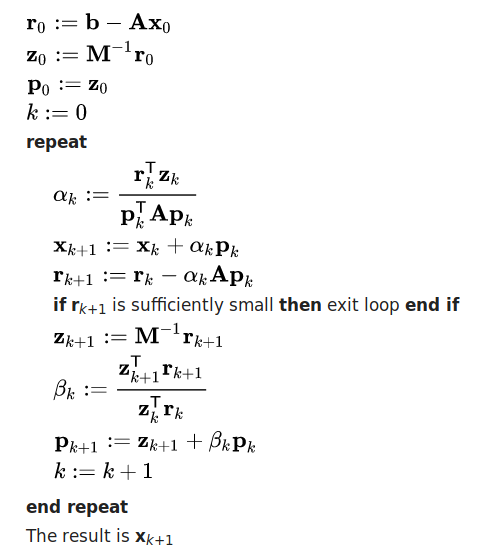
\includegraphics[width=7cm]{images/solvers/pcgwiki}}
\end{minipage}\hfill
\begin{minipage}{0.50\textwidth}
The same algorithm with our notations:\\
$\vec{r}_0 = \underline{\vec{f}} - \SSS \cdot \vec{\cal P}_0$\\
$\vec{z}_0= {\bm M}^{-1} \cdot \vec{r}_0$ \\
$\vec{p}_0 = \vec{z}_0$\\
$k=0$ \\
repeat\\
\hspace{8mm} $\alpha_k = (\vec{r}_k^T\cdot \vec{z}_k )/(\vec{p}_k \cdot \SSS\cdot  \vec{p}_k )$\\
\hspace{8mm} $\vec{\cal P}_{k+1} = \vec{\cal P}_k+\alpha_k \vec{p}_k$\\
\hspace{8mm} $\vec{r}_{k+1} = \vec{r}_k - \alpha_k \; \SSS \cdot \vec{p}_k $ \\
\hspace{8mm} $\vec{z}_{k+1} = {\bm M}^{-1} \cdot \vec{r}_{k+1}$ \\
\hspace{8mm} $\beta_k=(\vec{z}_{k+1}^T \cdot \vec{r}_{k+1})/(\vec{z}_k^T \cdot \vec{r}_k)$ \\
\hspace{8mm} $\vec{p}_{k+1} =\vec{z}_{k+1}+ \beta_k \vec{p}_k$ \\
$k=k+1$ \\
end repeat\\
return $\vec{\cal P}_{k+1}$ as the result
\end{minipage}

\vspace{.5cm}

Unsurprisingly we find the same algorithm in Saad \cite{saad}:

\frame{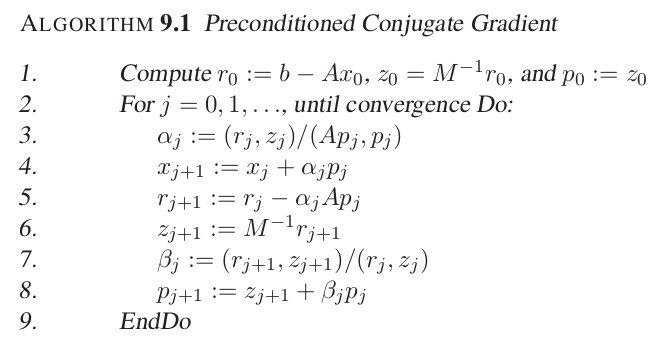
\includegraphics[width=7cm]{images/solvers/saad}}

Note that in the algorithm above the preconditioner matrix ${\bm M}$ 
has to be symmetric positive-definite and fixed, i.e., cannot change from iteration to iteration. 
We see that this algorithm introduces an additional vector $\vec{z}$ and a solve with the 
matrix ${\bm M}$ at each iteration, which means that ${\bm M}$ must 
be such that solving ${\bm M}\cdot \vec{x}= \vec{f}$ 
where $\vec{f}$ is a given rhs vector must be cheap. Ultimately, the PCG algorithm applied to 
the Schur complement equation takes the form:

\begin{mdframed}[backgroundcolor=blue!5]
\underline{\bf solver\_pcg}: assume $\vec{\cal P}_0$ known
\begin{itemize}
\item compute ${\cal V}_0=\K^{-1}(f-\G{\cal P}_0)$
\item $\vec{r}_0 = \G^T {\cal V}_0 - \C \cdot \vec{\cal P}_0 - \vec{h}$
\item if $\vec{r}_0$ is sufficiently small, then return $(\vec{\cal V}_0,\vec{\cal P}_0)$ as the result
\item $\vec{z}_0= M^{-1} \cdot \vec{r}_0$ 
\item $\vec{p}_0=\vec{z}_0$
\item $k=0$
\item repeat
\begin{itemize}
\item compute $\tilde{\vec{p}}_k = \G \cdot \vec{p}_k$
\item solve $\K\cdot  \vec{d}_k = \tilde{\vec{p}}_k$
\item compute $\alpha_k=(\vec{r}_k^T \cdot \vec{z}_k)/(\tilde{\vec{p}}_k^T \cdot \vec{d}_k
      + \vec{p}_k\cdot\C \cdot \vec{p}_k$)
\item $\vec{\cal P}_{k+1} = {\cal P}_k+\alpha_k \vec{p}_k$
\item $\vec{\cal V}_{k+1} = {\cal V}_k - \alpha_k \vec{d}_k$
\item $\vec{r}_{k+1} = \vec{r}_k - \alpha_k (\G^T \cdot \vec{d}_k + \C \cdot \vec{p}_k) $
\item if $\vec{r}_{k+1}$ is sufficiently small (i.e. $||\vec{r}_{k+1}||_2/||\vec{r}_0||_2 <tol$), 
      then exit loop
\item $\vec{z}_{k+1}=M^{-1} \cdot \vec{r}_{k+1}$
\item $\beta_k=(\vec{z}_{k+1}^T \cdot  \vec{r}_{k+1})/(\vec{z}_k^T \cdot  \vec{r}_k)$
\item $\vec{p}_{k+1} =\vec{z}_{k+1}+ \beta_k \vec{p}_k$
\item $k=k+1$
\end{itemize}
\item return $\vec{\cal P}_{k+1}$ as result
\end{itemize}
\end{mdframed}

Following Zhong \etal \cite{zhym12} one can define the following matrix as preconditioner:
\[
{\bm M} = diag \left[ \G^T (diag [\K]  )^{-1} \G \right]
\]
which is the preconditioner used for the Citcom codes (see appendix \ref{app:codes}). It 
can be constructed while the FEM matrix is being built/assembled
and it is trivial to invert. The entries in
$diag[\K]$ are the average viscosity in the elements associated
with a given degree of freedom.

Another very cheap way of building ${\bm M}$ for $Q_1\times P_0$ lements 
is to realise that the matrix $\SSS$ has dimensions element surface/volume 
divided by viscosity. We can then postulate 
\[
M_{e,e} = \frac{|\Omega|_e}{\eta_e} 
\]
where $e$ is an element and $\eta_e$ is the (average viscosity) inside the element.
For higher order elements, we need to use the pressure mass matrix.

These two preconditioners and two other variants are implemented in \stone 16 for 
$Q_1\times P_0$ elements.

%......................................................
\subsubsection{Generalized Conjugate Residual approach (Geenen \etal (2009))}

This approach is presented in Geenen \etal (2009) \cite{geum09}. 
The saddle point problem arising from the constrained Stokes equation is 
solved with a Krylov method, GCR \cite{vavu94}, right preconditioned (postconditioned) 
with a block triangular preconditioner (BTR) \cite{brpa88}.

The preconditioner ${\bm P}$ is given by
\[
{\bm P} = \left(
\begin{array}{cc}
\K & \G \\
0 & - \tilde{\SSS}
\end{array}
\right)
\]

The GCR algorithm \cite{eies83} in this case is taken from Vuik \etal (2000) \cite{vusb00}
and makes use of the block triangular preconditioner as follows:
\begin{itemize}
\item[] $\vec{r}_0 = \vec{b} - {\bm A}\cdot \vec{x}^0$
\item[] for $k$=0,1,2,...
\begin{itemize}
\item $\vec{s}^{k+1}={\bm P}^{-1} \cdot \vec{r}^k$
\item $\vec{v}^{k+1} = {\bm A}\cdot \vec{s}^{k+1}$
\item for i=0,1,...$k$
\begin{itemize}
\item $\vec{v}^{k+1}=\vec{v}^{k+1} - (\vec{v}^{k+1},\vec{v}^{i}) \vec{v}^i$
\item $\vec{s}^{k+1}=\vec{s}^{k+1} - (\vec{v}^{k+1},\vec{v}^{i}) \vec{s}^i$
\end{itemize}
\item end for
\item $\vec{v}^{k+1}=\vec{v}^{k+1} / \| \vec{v}^{k+1} \|_2$
\item $\vec{s}^{k+1}=\vec{s}^{k+1} / \| \vec{v}^{k+1} \|_2$  
\item $\vec{x}^{k+1} = \vec{x}^k + (\vec{v}^{k+1},\vec{r}^k) \vec{s}^{k+1} $
\item $\vec{r}^{k+1} = \vec{r}^k - (\vec{v}^{k+1}, \vec{r}^k) \vec{v}^{k+1}$
\end{itemize}
\item[] end for
\end{itemize}

As explained in Geenen \etal, instead of constructing ${\bm P}^{-1}$
explicitely and applying it to $\vec{r}$, we instead solve the system 
${\bm P}\cdot \vec{s} = \vec{r}$. We first decompose $\vec{r}$ and $\vec{s}$
as follows:
\[
\vec{r}^k = \left( \begin{array}{c} \vec{r}_\upnu^k \\ \vec{r}_p^k   \end{array} \right)
\qquad
\vec{s}^{k+1} = \left( \begin{array}{c} \vec{s}_\upnu^{k+1} \\ \vec{s}_p^{k+1}   \end{array} \right)
\]
so that we have to solve 
\[
\left(
\begin{array}{cc}
\K & \G \\
0 & - \tilde{\SSS}
\end{array}
\right)
\cdot
\left( \begin{array}{c} \vec{s}_\upnu^{k+1} \\ \vec{s}_p^{k+1}   \end{array} \right)
=
\left( \begin{array}{c} \vec{r}_\upnu^k \\ \vec{r}_p^k   \end{array} \right)
\]
This is actually rather trivial because of the upper triangular nature of the preconditioner ${\bm P}$.
It immediately follows:
\begin{eqnarray}
\tilde{\SSS}\cdot  \vec{s}_p^{k+1} &=& -\vec{r}_p^k   \\
\K \cdot \vec{s}_\upnu^{k+1} &=& \vec{r}_\upnu^k - \G \cdot \vec{s}_p^{k+1}
\end{eqnarray}
As before we now must specify how we solve the above two equations (and we must therefore
make a choice about the approximate Schur complement $\tilde{\SSS}$).

In the paper they take ${\bm  M}_p$, the pressure mass matrix scaled with the inverse of viscosity 
as an approximation to the Schur complement $\tilde{\SSS}$, which is spectrally equivalent.
Note that sometimes this mass matrix can be lumped which makes solving with it trivial and fast.

The inner solve with $\K$ is carried out with a CG solvers preconditioned with AMG. They 
state that ``Using AMG as a preconditioner to CG for the subsystem solution
guarantees $h$-independent convergence of the solver during the preconditioner construction phase.''

%......................................................
\subsubsection{Using MINRES a la Burstedde \etal (2008)}

This approach is presented in Burstedde \etal (2008) \cite{bugg08}.
They state that neglecting the off-diagonal blocks motivates use of the symmetric
positive definite preconditioner:
\[
{\bm P} = \left(
\begin{array}{cc}
\tilde{\K} & 0 \\
0 & \tilde{\SSS}
\end{array}
\right)
\]
where $\tilde{\K}$ is a variable-viscosity discrete vector Laplacian
approximation of $\K$ (see explanations in \cite{bugs09}), 
which is motivated by the fact that
for constant viscosity and Dirichlet boundary conditions,
$\K$ and $\tilde\K$ are equivalent. 
$\tilde{\SSS}$ is an approximation of
the Schur complement given by a lumped mass matrix
weighted by the inverse viscosity $\eta^{-1}$. The resulting
diagonal matrix $\tilde{\SSS}$ is spectrally equivalent to $\SSS$ \cite{elsw}.
They also use AMG as preconditioner for the inner solves. 

Note that Burstedde \etal  (2008) \cite{bugg08} relies on stabilised 
$Q_1\times Q_1$ elements from Dohrmann \& Bochev \cite{dobo04} 
so that their Stokes matrix does feature the associated $-\C$ block.
Subsequent papers do so too, see Burstedde \etal (2009) \cite{bugs09}, 
Burstedde \etal (2013) \cite{busa13}.
The same solver structure based on MINRES is used in these articles too.

%---------------------------------------------
\subsubsection{The Augmented Lagrangian approach}
\index{general}{Augmented Lagrangian}

see LaCoDe paper \cite{demh19}.

We start from the saddle point Stokes system:
\begin{equation}
\left(
\begin{array}{cc}
\K & \G \\ \G^T & 0 
\end{array}
\right)
\cdot
\left(
\begin{array}{c}
\vec{\cal V} \\ \vec{\cal P}
\end{array}
\right)
=
\left(
\begin{array}{c}
\vec{f} \\ \vec{h}
\end{array}
\right)
\label{StokesSyst2}
\end{equation}
The AL method consists of subtracting $\lambda^{-1} \mathbb{M}_p \cdot \vec{\cal P}$ from the left and 
right-side of the mass conservation equation (where $\mathbb{M}_p$ is the pressure mass matrix) 
and introducing the following iterative scheme:
\begin{equation}
\left(
\begin{array}{cc}
\K & \G \\ \G^T & -\lambda^{-1} \mathbb{M}_p
\end{array}
\right)
\cdot
\left(
\begin{array}{c}
\vec{\cal V}^{k+1} \\ \vec{\cal P}^{k+1}
\end{array}
\right)
=
\left(
\begin{array}{c}
\vec{f} \\ \vec{h} - \lambda^{-1} \mathbb{M}_p \cdot \vec{\cal P}^k
\end{array}
\right)
\label{ALStokes}
\end{equation}
where $k$ is the iteration counter and $\lambda$ is an artificial compressibility term which has 
the dimensions of dynamic viscosity. 
The choice of $\lambda$ can be difficult as too low or too high a value yields either erroneous results and/or terribly ill-conditioned matrices. LaCoDe paper (!!) use such a method and report that $\lambda=\max_\Omega({\eta})$
works well. 
Note that at convergence we have $||\vec{\cal P}^{k+1}-\vec{\cal P}^k||<\epsilon$ and then Eq.(\ref{ALStokes}) converges to Eq.(\ref{StokesSyst2}) and the velocity and pressure fields are solution of the unmodified system Eq.(\ref{StokesSyst2}).

The introduction of this term serves one purpose: allowing us to solve the system in a segregated manner (i.e. computing successive iterates of the velocity and pressure fields until convergence is reached).
The second line of Eq.~(\ref{ALStokes}) is 
\[
\G^T \cdot \vec{\cal V}^{k+1} - \lambda^{-1} \mathbb{M}_p \cdot \vec{\cal P}^{k+1} = \vec{h} - \lambda^{-1} \mathbb{M}_p \cdot \vec{\cal P}^k
\]
and can therefore be rewritten
\[
\vec{\cal P}^{k+1} = \vec{\cal P}^k + \lambda \mathbb{M}_p^{-1} \cdot (\G^T \cdot \vec{\cal V}^{k+1} - \vec h)
\]
We can then substitute this expression of $\vec{\cal P}^{k+1}$ in the first equation. This yields:
\begin{eqnarray}
\K \cdot \vec{\cal V}^{k+1}  
&=& \vec f - \G \cdot {\cal P}^{k+1}) \\
\K \cdot \vec{\cal V}^{k+1}  
&=& \vec f - \G \cdot ( \vec{\cal P}^k + \lambda \mathbb{M}_p^{-1} \cdot  (\G^T \cdot \vec{\cal V}^{k+1} - \vec h)  ) \\
\K \cdot \vec{\cal V}^{k+1} + \lambda \G \cdot \mathbb{M}_p^{-1} \cdot \G^T \cdot \vec{\cal V}^{k+1} 
&=& \vec f - \G \cdot ( \vec{\cal P}^k - \lambda \mathbb{M}_p^{-1}\vec h)  ) \\
\underbrace{  \left(  \K  + \lambda \G \cdot \mathbb{M}_p^{-1} \cdot \G^T \right)   }_{\tilde{\K}  } \cdot \vec{\cal V}^{k+1} 
&=& \underbrace{ \vec f - \G \cdot ( \vec{\cal P}^k - \lambda \mathbb{M}_p^{-1}\vec h)  )}_{\vec{f}^{k+1}} \\
\end{eqnarray}
The iterative algorithm goes as follows:
\begin{mdframed}[backgroundcolor=blue!5]
\begin{enumerate}
\item if it is the first timestep, set $\vec{\cal P}^0=0$ , otherwise set it to the pressure of the previous timestep.
\item calculate $\tilde{\K}$
\item calculate $\vec{f}^{k+1}$
\item solve $\tilde{\K} \cdot \vec{\cal V}^{k+1} = \vec{f}^{k+1}$
\item update pressure with 
$\vec{\cal P}^{k+1} = \vec{\cal P}^k + \lambda \mathbb{M}_p^{-1} \cdot (\G^T \cdot \vec{\cal V}^{k+1} - \vec h)$
\end{enumerate}
\end{mdframed}

\begin{remark} 
If discontinuous pressures are used, the pressure mass matrix can be inverted element by element which is 
cheaper than inverting $\mathbb{M}_p$ as a whole.
\end{remark}

\begin{remark} 
This method has obvious ties with the penalty method. 
\end{remark}

\begin{remark} 
If $\lambda >> \max_\Omega{\eta}$ then the matrix $\tilde{\K}$ is ill-conditioned and an iterative solver must be used.
\end{remark}

%------------------------------------------------------------------------------
\subsubsection{The SIMPLE method}

The SIMPLE method (Semi-Implicit Method for Pressure-Linked Equations)
has been introduced by Patankar \& Spalding (1972) \cite{pasp72} as an iterative method to solve
the finite volume discretized incompressible Navier-Stokes equations. 
%The algorithm
%is based on the following steps:
%\begin{itemize}
%\item First the pressure is assumed to be known from the previous iteration.
%\item Then the velocity is solved from the momentum equations. The newly obtained
%velocities do not satisfy the continuity equation since the pressure is only a
%guess.
%\item In the next substeps the velocities and pressures are corrected in order to
%satisfy the discrete continuity equation.
%\end{itemize}
In a nutshell, the algorithm follows from a block LU decomposition
\begin{equation}
\left(
\begin{array}{cc}
\K & \G \\ \G^T & -\C 
\end{array}
\right)
\cdot
\left(
\begin{array}{c}
\vec{\cal V} \\ \vec{\cal P}
\end{array}
\right)
=
\left(
\begin{array}{cc}
\K & 0 \\ 
\G^T & -\SSS
\end{array}
\right)
\cdot
\left(
\begin{array}{cc}
{\bm I} & \K^{-1} \cdot \G \\
0 & {\bm I} 
\end{array}
\right)
\cdot
\left(
\begin{array}{c}
\vec{\cal V} \\ \vec{\cal P}
\end{array}
\right)
=
\left(
\begin{array}{c}
\vec{f} \\ \vec{h}
\end{array}
\right)
\end{equation}
The approximation $\K^{-1}$ as ${\bm D}_\K^{-1} = (diag(\K))^{-1}$ leads to the 
SIMPLE algorithm. In this case the approximation of the Schur complement matrix is given by
$\tilde{\SSS} = \G^T\cdot  {\bm D}_\K^{-1} \cdot \G$  and the decomposition looks like
\[
\left(
\begin{array}{cc}
\K & \G \\ \G^T & -\C 
\end{array}
\right)
\simeq
\left(
\begin{array}{cc}
\K & 0 \\ 
\G^T & -\tilde{\SSS}
\end{array}
\right)
\cdot
\left(
\begin{array}{cc}
{\bm I} & {\bm D}_\K^{-1} \cdot \G \\
0 & {\bm I} 
\end{array}
\right)
\]

Before we can write out the SIMPLE algorithm, we must first take a small detour via so-called
distributive iterative methods \cite{vusb00,tack10}. \index{general}{Distributive Iterative Method}
Let us consider the linear system 
\[
{\bm A}\cdot \vec{x}=\vec{b}
\] 
A stationary iterative method is defined as follows:
\[
\vec{x}^{k+1}= {\bm B}\cdot \vec{x}^{k}+ \vec{c}
\]
where $\vec{c}=({\bm I}-{\bm B})\cdot {\bm A}^{-1}\cdot \vec{b}$. 
Left-multiplying all terms by $({\bm I}-{\bm B})^{-1}$ first and then left-multiplying again 
by ${\bm A}$  we arrive at:
\[
{\bm A}\cdot ({\bm I}-{\bm B})^{-1}\cdot \vec{x}^{k+1}
={\bm A}\cdot ({\bm I}-{\bm B})^{-1}\cdot {\bm B}\cdot 
\vec{x}^{k} + {\bm A}\cdot ({\bm I}-{\bm B})^{-1} \cdot \vec{c}
\]
We define ${\bm M}={\bm A}\cdot ({\bm I}-{\bm B})^{-1} $ so that now
\[
{\bm M}\cdot\vec{x}^{k+1}={\bm M}\cdot {\bm B}\cdot \vec{x}^{k}+\vec{b} 
\]
We define ${\bm N}={\bm M}\cdot {\bm B}$
and finally 
\[
{\bm M}\cdot\vec{x}^{k+1}={\bm N}\cdot \vec{x}^{k}+\vec{b} 
\]
Note that ${\bm M}-{\bm N}={\bm M}-{\bm M}\cdot {\bm B}
= {\bm M}\cdot  ({\bm I}-{\bm B}) 
= {\bm A}\cdot ({\bm I}-{\bm B})^{-1}\cdot ({\bm I}-{\bm B}) 
= {\bm A}$. 
Let us now write the original system 
${\bm A}\cdot \vec{x}=\vec{b}$ as $({\bm A}\cdot {\bm B})\cdot ({\bm B}^{-1}\cdot \vec{x})=\vec{b}$
or, $ \underline{\bm A}\cdot  \underline{\vec{x}}=\vec{b} $
with 
$\vec{x}={\bm B}\cdot \underline{\vec{x}}$
and 
$\underline{\bm A}={\bm A}\cdot {\bm B}$.
Splitting $\underline{\bm A}={\bm M}-{\bm N}$ again yields 
\[
{\bm M}\cdot \underline{\vec{x}}^{k+1}={\bm N}\cdot \underline{\vec{x}}^{k}+\vec{b} 
\]
Using $\vec{x}={\bm B}\cdot \underline{\vec{x}}$, we get 
\[
{\bm M}\cdot {\bm B}^{-1}\cdot \vec{x}^{k+1} = {\bm N}\cdot {\bm B}^{-1}\cdot  \vec{x}^{k}+\vec{b} 
\]
We then have 
\begin{eqnarray}
\vec{x}^{k+1}
&=&  {\bm B}\cdot {\bm M}^{-1} \cdot[ {\bm N} \cdot  {\bm B}^{-1}  \cdot \vec{x}^{k}+ \vec{b}  ] \\
&=&  {\bm B}\cdot {\bm M}^{-1} \cdot[ ({\bm M} - \underline{\bm A}) \cdot  {\bm B}^{-1}\cdot \vec{x}^{k}+\vec{b}  ]\\
&=&  {\bm B}\cdot {\bm M}^{-1} \cdot[ ({\bm M} - {\bm A}\cdot {\bm B}) \cdot  {\bm B}^{-1}\cdot  \vec{x}^{k}+ \vec{b}  ]\\
&=&  {\bm B}\cdot {\bm M}^{-1} \cdot[ {\bm M}\cdot {\bm B}^{-1} \cdot \vec{x}^{k} - {\bm A}\cdot {\bm B}\cdot  {\bm B}^{-1} \cdot \vec{x}^{k}+\vec{b}  ]\\
&=&  {\bm B}\cdot {\bm M}^{-1} \cdot[ {\bm M}\cdot {\bm B}^{-1} \cdot \vec{x}^{k} - {\bm A}\cdot \vec{x}^{k}+ \vec{b}  ]\\
&=&  \vec{x}^k + {\bm B}\cdot {\bm M}^{-1}\cdot [ \vec{b}    - {\bm A} \cdot \vec{x}^{k}  ]
\end{eqnarray}
Finally, we have the following recursion:
\begin{equation}
\boxed{\vec{x}^{k+1} = \vec{x}^k +{\bm B} \cdot {\bm M} ^{-1}\cdot (\vec{b} -{\bm A}\cdot \vec{x}^{k}  ) }
\label{eq:simplerec}
\end{equation}
Coming back to the SIMPLE algorithm, we start from 
\[
{\bm A}=
\left(
\begin{array}{cc}
\K & \G \\
\G^T & 0
\end{array}
\right)
\]
The matrix ${\bm B}$ is then chosen to be 
\[
{\bm B}=
\left(
\begin{array}{cc}
{\bm I} & -\K^{-1} \G \\
0 & {\bm I}
\end{array}
\right)
\]
We then have 
\[
{\bm A}\cdot  {\bm B} = 
\left(
\begin{array}{cc}
\K & \G \\
\G^T & 0
\end{array}
\right)
\cdot 
\left(
\begin{array}{cc}
{\bm I} & -\K^{-1} \G \\
0 & {\bm I}
\end{array}
\right)
=
\left(
\begin{array}{cc}
\K & 0 \\
\G^T & -\SSS
\end{array}
\right)
\]
where $\SSS=\G^T\K^{-1}\G$.
Let us recall that we define ${\bm D}_\K =diag(\K)$ and $\hat{\SSS}=\G^T \cdot {\bm D}_\K^{-1} \cdot \G$. 
We further define 
\[
{\bm M}=
\left(
\begin{array}{cc}
\K & 0 \\
\G^T & -\hat{\SSS}
\end{array}
\right)
\]
and ${\bm N}$ follows from the splitting ${\bm A}\cdot {\bm B}= {\bm M} - {\bm N}$. 
(Note that we do not need to form nor use ${\bm N}$).

The standard SIMPLE algorithm also replaces $\K^{-1}$  by  ${\bm D}_\K^{-1}$ in ${\bm B}$ so that 
${\bm B}$ is approximated by:
\[
{\bm B}=
\left(
\begin{array}{cc}
{\bm I} & -{\bm D}_\K^{-1} \G \\
0 & {\bm I}
\end{array}
\right)
\]
in the iterations.
We can define 
\[
\vec{r}^k=
\vec{b}-{\bm A}\cdot \vec{x}^k = 
\left(
\begin{array}{c}
\vec{f} \\ \vec{h}
\end{array}
\right)
-
\left(
\begin{array}{cc}
\K & \G \\
\G^T & 0
\end{array}
\right)
\cdot
\left(
\begin{array}{c}
\vec{\cal V}^k \\ \vec{\cal P}^k
\end{array}
\right)
=
\left(
\begin{array}{c}
\vec{r}_{\cal V}^k \\ \vec{r}_{\cal P}^k
\end{array}
\right)
\]

The iteration loop of Eq.~\eqref{eq:simplerec} then takes the form 
\[
\left(
\begin{array}{c}
\vec{\cal V}^{k+1} \\ 
\vec{\cal P}^{k+1}
\end{array}
\right)
=
\left(
\begin{array}{c}
V^k \\ P^k
\end{array}
\right)
+ 
{\bm B}  {\bm M} ^{-1}
\left(
\begin{array}{c}
r_V^k \\ r_P^k
\end{array}
\right)
=
\left(
\begin{array}{c}
V^k \\ P^k
\end{array}
\right)
+ 
\left(
\begin{array}{c}
\delta V^k \\ \delta P^k
\end{array}
\right)
\quad\quad
\textrm{with}\quad\quad
\left(
\begin{array}{c}
\delta V^k \\ \delta P^k
\end{array}
\right)
=
{\bm B}  {\bm M} ^{-1}
\left(
\begin{array}{c}
\vec{r}_{\cal V}^k \\ 
\vec{r}_{\cal P}^k
\end{array}
\right)
\]
This last equation can be rewritten\footnote{Remember 
that $({\bm A}\cdot {\bm B})^{-1}={\bm B}^{-1}\cdot {\bm A}^{-1}$}:
\[
{\bm M} \cdot 
\left[ {\bm B}^{-1} \cdot 
\left(
\begin{array}{c}
\delta \vec{\cal V}^k \\ 
\delta \vec{\cal P}^k
\end{array}
\right)
\right]
=
\left(
\begin{array}{c}
\vec{r}_{\cal V}^k \\ 
\vec{r}_{\cal P}^k
\end{array}
\right)
\]
We then have to solve 
\begin{equation}
{\bm M} 
\cdot
\left(
\begin{array}{c}
\delta^\star \vec{\cal V}^k \\ 
\delta^\star \vec{\cal P}^k
\end{array}
\right)
=
\left(
\begin{array}{cc}
\K & 0 \\
\G^T & -\hat{\SSS}
\end{array}
\right)
\cdot
\left(
\begin{array}{c}
\delta^\star \vec{\cal V}^k \\ 
\delta^\star \vec{\cal P}^k
\end{array}
\right)
=
\left(
\begin{array}{c}
\vec{r}_{\cal V}^k \\ 
\vec{r}_{\cal P}^k
\end{array}
\right)
\label{simple1aa}
\end{equation}
and then compute
\begin{equation}
\left(
\begin{array}{c}
\delta \vec{\cal V}^k \\ 
\delta \vec{\cal P}^k
\end{array}
\right)
=
{\bm B}  
\left(
\begin{array}{c}
\delta^\star \vec{\cal V}^k \\ 
\delta^\star \vec{\cal P}^k
\end{array}
\right)
\label{simple2aa}
\end{equation}
Fortunately Eq.~\eqref{simple1aa} translates into:
\begin{eqnarray}
\K \cdot \delta^\star \vec{\cal V}^k &=&  \vec{r}_{\cal V}^k   \\
\hat{\SSS} \cdot  \delta^\star \vec{\cal P}^k &=&  - \vec{r}_P^k + \G^T \cdot \delta^\star \vec{V}^k 
\end{eqnarray}
and Eq.~\eqref{simple2aa} translates into:
\[
\left(
\begin{array}{c}
\delta \vec{\cal V}^k \\ 
\delta \vec{\cal P}^k
\end{array}
\right)
=
\left(
\begin{array}{cc}
{\bm I} & -{\bm D}_\K^{-1}\cdot \G \\
0 & {\bm I}
\end{array}
\right)
\cdot
\left(
\begin{array}{c}
\delta^\star \vec{\cal V}^k \\ 
\delta^* \vec{\cal P}^k
\end{array}
\right)
\]
or, 
\begin{eqnarray}
\delta \vec{\cal V}_k &=& \delta^\star \vec{\cal V}^k 
-{\bm D}_\K^{-1}\cdot \G \cdot\delta^\star \vec{\cal P}_k \\
\delta \vec{\cal P}_k &=& \delta^\star \vec{\cal P}^k
\end{eqnarray}

\newpage
The final algorithm will then look as follows:

\begin{mdframed}[backgroundcolor=blue!5]
\begin{enumerate}
\item compute the residuals 
\begin{eqnarray}
\vec{r}_{\cal V} &=& \vec{f} - \K \cdot \vec{\cal V}^{(k)} - \G \cdot \vec{\cal P}^{(k)} \nn\\
\vec{r}_{\cal P} &=& \vec{h} - \G^T \cdot \vec{\cal V}^{(k)}
\end{eqnarray}
\item Solve $\K  \cdot \delta^\star \vec{\cal V}^k =  \vec{r}_{\cal V}^k  $
\item Solve $\hat{\SSS} \cdot \delta^\star \vec{\cal P}^k =  \vec{r}_{\cal P}^k - \G^T \cdot  \delta^\star V^k $
\item Compute $\delta \vec{\cal V}^k = \delta^\star \vec{\cal V}^k -{\bm D}_\K^{-1} \cdot \G \cdot \delta^\star \vec{\cal P}_k $
\item Update $\delta \vec{\cal P}^k = \delta^\star \vec{\cal P}^k$
\item Update 
\begin{eqnarray}
\vec{\cal V}^{(k+1)} &=& \vec{\cal V}^{(k)} + \omega_{\cal V} \delta \vec{\cal V}^{(k)} \nn\\
\vec{\cal P}^{(k+1)} &=& \vec{\cal P}^{(k)} + \omega_{\cal P} \delta \vec{\cal P}^{(k)} 
\end{eqnarray}
\end{enumerate}
\end{mdframed}
where the parameters $\omega_{\cal V}$ and $\omega_{\cal P}$ are between 0 and 1. 

\Literature: Echevarria Serur (2013) \cite{eche13}, Braess \& Sarazin (1997) \cite{brsa97b}, 
see Ur Rehman \etal (2009) \cite{urvs09} for SIMPLE(R) algorithm. See also \cite{tack10}.
















%...................................................
\subsubsection{The GMRES approach - NOT FINISHED}

The Generalized Minimal Residual method \cite{sasc86} 
is an extension of MINRES (which is only applicable to symmetric systems) to unsymmetric systems. 
Like MINRES, it generates a sequence of orthogonal vectors and 
combines these through a least-squares solve and update. However, 
in the absence of symmetry this can no longer be done with short recurrences. As a consequence, 
all previously computed vectors in the orthogonal sequence have to be retained and 
for this reason ''restarted'' versions of the method are used.

It must be said that the (preconditioned) GMRES method is actually much more difficult to implement 
than the (preconditioned) Conjugate Gradient method.
However, since it can deal with unsymmetric matrices, it means that it can be applied 
directly to the Stokes system matrix (as opposed to the CG method which is used on the Schur complement
equation).

 
%In what follows we wish to solve the linear system ${\bm A}\cdot \vec x = \vec b$ and use the preconditioner 
%matrix ${\bm M}$.

\Literature: \cite[p208]{eijkhout} \cite{saad,saad93} \cite{babc94} \cite{ayac03}

\todo[inline]{finish GMRES algo description. not sure what to do, hard to explain, not easy to code.}

%Let $\vec x^{(0)}$ be an initial guess of the solution.

%for j=1,2,...

%    solve $\vec r$ from ${\bm M}\cdot \vec r = \vec b - {\bm A}\cdot \vec x^{(0)}$

%    $\vec v^{(1)}=\vec{r}/||\vec r||_2$

%    $\vec s = ||\vec r||_2 \; \vec e_1$

%    for i=1,2,...m
 
%        solve $\vec w$ from $\bm M \cdot \vec w = \bm A \cdot \vec v^{(i)}$

%        for k=1,...i

%            $h_{k,i}=(\vec w,\vec v^{(k)})$

%            $\vec w=\vec w-h_{k,i} \vec v^{(k)}$

%        end 

%        $h_{i+1,i}=||\vec w||_2$

%        $\vec v^{(i+1)} = \vec w/h_{i+1,i}$

%end 



the FGMRES approach \cite{deit13}

\Literature \cite{pasa75,mamo08,fumt11,knke04,kool00,kopo93} 

